\documentclass{article}
\usepackage{iclr2027_conference,times}
\usepackage[T1]{fontenc}
%%%%% NEW MATH DEFINITIONS %%%%%

\usepackage{amsmath,amsfonts,bm}

% Mark sections of captions for referring to divisions of figures
\newcommand{\figleft}{{\em (Left)}}
\newcommand{\figcenter}{{\em (Center)}}
\newcommand{\figright}{{\em (Right)}}
\newcommand{\figtop}{{\em (Top)}}
\newcommand{\figbottom}{{\em (Bottom)}}
\newcommand{\captiona}{{\em (a)}}
\newcommand{\captionb}{{\em (b)}}
\newcommand{\captionc}{{\em (c)}}
\newcommand{\captiond}{{\em (d)}}

% Highlight a newly defined term
\newcommand{\newterm}[1]{{\bf #1}}


% Figure reference, lower-case.
\def\figref#1{figure~\ref{#1}}
% Figure reference, capital. For start of sentence
\def\Figref#1{Figure~\ref{#1}}
\def\twofigref#1#2{figures \ref{#1} and \ref{#2}}
\def\quadfigref#1#2#3#4{figures \ref{#1}, \ref{#2}, \ref{#3} and \ref{#4}}
% Section reference, lower-case.
\def\secref#1{section~\ref{#1}}
% Section reference, capital.
\def\Secref#1{Section~\ref{#1}}
% Reference to two sections.
\def\twosecrefs#1#2{sections \ref{#1} and \ref{#2}}
% Reference to three sections.
\def\secrefs#1#2#3{sections \ref{#1}, \ref{#2} and \ref{#3}}
% Reference to an equation, lower-case.
\def\eqref#1{equation~\ref{#1}}
% Reference to an equation, upper case
\def\Eqref#1{Equation~\ref{#1}}
% A raw reference to an equation---avoid using if possible
\def\plaineqref#1{\ref{#1}}
% Reference to a chapter, lower-case.
\def\chapref#1{chapter~\ref{#1}}
% Reference to an equation, upper case.
\def\Chapref#1{Chapter~\ref{#1}}
% Reference to a range of chapters
\def\rangechapref#1#2{chapters\ref{#1}--\ref{#2}}
% Reference to an algorithm, lower-case.
\def\algref#1{algorithm~\ref{#1}}
% Reference to an algorithm, upper case.
\def\Algref#1{Algorithm~\ref{#1}}
\def\twoalgref#1#2{algorithms \ref{#1} and \ref{#2}}
\def\Twoalgref#1#2{Algorithms \ref{#1} and \ref{#2}}
% Reference to a part, lower case
\def\partref#1{part~\ref{#1}}
% Reference to a part, upper case
\def\Partref#1{Part~\ref{#1}}
\def\twopartref#1#2{parts \ref{#1} and \ref{#2}}

\def\ceil#1{\lceil #1 \rceil}
\def\floor#1{\lfloor #1 \rfloor}
\def\1{\bm{1}}
\newcommand{\train}{\mathcal{D}}
\newcommand{\valid}{\mathcal{D_{\mathrm{valid}}}}
\newcommand{\test}{\mathcal{D_{\mathrm{test}}}}

\def\eps{{\epsilon}}


% Random variables
\def\reta{{\textnormal{$\eta$}}}
\def\ra{{\textnormal{a}}}
\def\rb{{\textnormal{b}}}
\def\rc{{\textnormal{c}}}
\def\rd{{\textnormal{d}}}
\def\re{{\textnormal{e}}}
\def\rf{{\textnormal{f}}}
\def\rg{{\textnormal{g}}}
\def\rh{{\textnormal{h}}}
\def\ri{{\textnormal{i}}}
\def\rj{{\textnormal{j}}}
\def\rk{{\textnormal{k}}}
\def\rl{{\textnormal{l}}}
% rm is already a command, just don't name any random variables m
\def\rn{{\textnormal{n}}}
\def\ro{{\textnormal{o}}}
\def\rp{{\textnormal{p}}}
\def\rq{{\textnormal{q}}}
\def\rr{{\textnormal{r}}}
\def\rs{{\textnormal{s}}}
\def\rt{{\textnormal{t}}}
\def\ru{{\textnormal{u}}}
\def\rv{{\textnormal{v}}}
\def\rw{{\textnormal{w}}}
\def\rx{{\textnormal{x}}}
\def\ry{{\textnormal{y}}}
\def\rz{{\textnormal{z}}}

% Random vectors
\def\rvepsilon{{\mathbf{\epsilon}}}
\def\rvtheta{{\mathbf{\theta}}}
\def\rva{{\mathbf{a}}}
\def\rvb{{\mathbf{b}}}
\def\rvc{{\mathbf{c}}}
\def\rvd{{\mathbf{d}}}
\def\rve{{\mathbf{e}}}
\def\rvf{{\mathbf{f}}}
\def\rvg{{\mathbf{g}}}
\def\rvh{{\mathbf{h}}}
\def\rvu{{\mathbf{i}}}
\def\rvj{{\mathbf{j}}}
\def\rvk{{\mathbf{k}}}
\def\rvl{{\mathbf{l}}}
\def\rvm{{\mathbf{m}}}
\def\rvn{{\mathbf{n}}}
\def\rvo{{\mathbf{o}}}
\def\rvp{{\mathbf{p}}}
\def\rvq{{\mathbf{q}}}
\def\rvr{{\mathbf{r}}}
\def\rvs{{\mathbf{s}}}
\def\rvt{{\mathbf{t}}}
\def\rvu{{\mathbf{u}}}
\def\rvv{{\mathbf{v}}}
\def\rvw{{\mathbf{w}}}
\def\rvx{{\mathbf{x}}}
\def\rvy{{\mathbf{y}}}
\def\rvz{{\mathbf{z}}}

% Elements of random vectors
\def\erva{{\textnormal{a}}}
\def\ervb{{\textnormal{b}}}
\def\ervc{{\textnormal{c}}}
\def\ervd{{\textnormal{d}}}
\def\erve{{\textnormal{e}}}
\def\ervf{{\textnormal{f}}}
\def\ervg{{\textnormal{g}}}
\def\ervh{{\textnormal{h}}}
\def\ervi{{\textnormal{i}}}
\def\ervj{{\textnormal{j}}}
\def\ervk{{\textnormal{k}}}
\def\ervl{{\textnormal{l}}}
\def\ervm{{\textnormal{m}}}
\def\ervn{{\textnormal{n}}}
\def\ervo{{\textnormal{o}}}
\def\ervp{{\textnormal{p}}}
\def\ervq{{\textnormal{q}}}
\def\ervr{{\textnormal{r}}}
\def\ervs{{\textnormal{s}}}
\def\ervt{{\textnormal{t}}}
\def\ervu{{\textnormal{u}}}
\def\ervv{{\textnormal{v}}}
\def\ervw{{\textnormal{w}}}
\def\ervx{{\textnormal{x}}}
\def\ervy{{\textnormal{y}}}
\def\ervz{{\textnormal{z}}}

% Random matrices
\def\rmA{{\mathbf{A}}}
\def\rmB{{\mathbf{B}}}
\def\rmC{{\mathbf{C}}}
\def\rmD{{\mathbf{D}}}
\def\rmE{{\mathbf{E}}}
\def\rmF{{\mathbf{F}}}
\def\rmG{{\mathbf{G}}}
\def\rmH{{\mathbf{H}}}
\def\rmI{{\mathbf{I}}}
\def\rmJ{{\mathbf{J}}}
\def\rmK{{\mathbf{K}}}
\def\rmL{{\mathbf{L}}}
\def\rmM{{\mathbf{M}}}
\def\rmN{{\mathbf{N}}}
\def\rmO{{\mathbf{O}}}
\def\rmP{{\mathbf{P}}}
\def\rmQ{{\mathbf{Q}}}
\def\rmR{{\mathbf{R}}}
\def\rmS{{\mathbf{S}}}
\def\rmT{{\mathbf{T}}}
\def\rmU{{\mathbf{U}}}
\def\rmV{{\mathbf{V}}}
\def\rmW{{\mathbf{W}}}
\def\rmX{{\mathbf{X}}}
\def\rmY{{\mathbf{Y}}}
\def\rmZ{{\mathbf{Z}}}

% Elements of random matrices
\def\ermA{{\textnormal{A}}}
\def\ermB{{\textnormal{B}}}
\def\ermC{{\textnormal{C}}}
\def\ermD{{\textnormal{D}}}
\def\ermE{{\textnormal{E}}}
\def\ermF{{\textnormal{F}}}
\def\ermG{{\textnormal{G}}}
\def\ermH{{\textnormal{H}}}
\def\ermI{{\textnormal{I}}}
\def\ermJ{{\textnormal{J}}}
\def\ermK{{\textnormal{K}}}
\def\ermL{{\textnormal{L}}}
\def\ermM{{\textnormal{M}}}
\def\ermN{{\textnormal{N}}}
\def\ermO{{\textnormal{O}}}
\def\ermP{{\textnormal{P}}}
\def\ermQ{{\textnormal{Q}}}
\def\ermR{{\textnormal{R}}}
\def\ermS{{\textnormal{S}}}
\def\ermT{{\textnormal{T}}}
\def\ermU{{\textnormal{U}}}
\def\ermV{{\textnormal{V}}}
\def\ermW{{\textnormal{W}}}
\def\ermX{{\textnormal{X}}}
\def\ermY{{\textnormal{Y}}}
\def\ermZ{{\textnormal{Z}}}

% Vectors
\def\vzero{{\bm{0}}}
\def\vone{{\bm{1}}}
\def\vmu{{\bm{\mu}}}
\def\vtheta{{\bm{\theta}}}
\def\va{{\bm{a}}}
\def\vb{{\bm{b}}}
\def\vc{{\bm{c}}}
\def\vd{{\bm{d}}}
\def\ve{{\bm{e}}}
\def\vf{{\bm{f}}}
\def\vg{{\bm{g}}}
\def\vh{{\bm{h}}}
\def\vi{{\bm{i}}}
\def\vj{{\bm{j}}}
\def\vk{{\bm{k}}}
\def\vl{{\bm{l}}}
\def\vm{{\bm{m}}}
\def\vn{{\bm{n}}}
\def\vo{{\bm{o}}}
\def\vp{{\bm{p}}}
\def\vq{{\bm{q}}}
\def\vr{{\bm{r}}}
\def\vs{{\bm{s}}}
\def\vt{{\bm{t}}}
\def\vu{{\bm{u}}}
\def\vv{{\bm{v}}}
\def\vw{{\bm{w}}}
\def\vx{{\bm{x}}}
\def\vy{{\bm{y}}}
\def\vz{{\bm{z}}}

% Elements of vectors
\def\evalpha{{\alpha}}
\def\evbeta{{\beta}}
\def\evepsilon{{\epsilon}}
\def\evlambda{{\lambda}}
\def\evomega{{\omega}}
\def\evmu{{\mu}}
\def\evpsi{{\psi}}
\def\evsigma{{\sigma}}
\def\evtheta{{\theta}}
\def\eva{{a}}
\def\evb{{b}}
\def\evc{{c}}
\def\evd{{d}}
\def\eve{{e}}
\def\evf{{f}}
\def\evg{{g}}
\def\evh{{h}}
\def\evi{{i}}
\def\evj{{j}}
\def\evk{{k}}
\def\evl{{l}}
\def\evm{{m}}
\def\evn{{n}}
\def\evo{{o}}
\def\evp{{p}}
\def\evq{{q}}
\def\evr{{r}}
\def\evs{{s}}
\def\evt{{t}}
\def\evu{{u}}
\def\evv{{v}}
\def\evw{{w}}
\def\evx{{x}}
\def\evy{{y}}
\def\evz{{z}}

% Matrix
\def\mA{{\bm{A}}}
\def\mB{{\bm{B}}}
\def\mC{{\bm{C}}}
\def\mD{{\bm{D}}}
\def\mE{{\bm{E}}}
\def\mF{{\bm{F}}}
\def\mG{{\bm{G}}}
\def\mH{{\bm{H}}}
\def\mI{{\bm{I}}}
\def\mJ{{\bm{J}}}
\def\mK{{\bm{K}}}
\def\mL{{\bm{L}}}
\def\mM{{\bm{M}}}
\def\mN{{\bm{N}}}
\def\mO{{\bm{O}}}
\def\mP{{\bm{P}}}
\def\mQ{{\bm{Q}}}
\def\mR{{\bm{R}}}
\def\mS{{\bm{S}}}
\def\mT{{\bm{T}}}
\def\mU{{\bm{U}}}
\def\mV{{\bm{V}}}
\def\mW{{\bm{W}}}
\def\mX{{\bm{X}}}
\def\mY{{\bm{Y}}}
\def\mZ{{\bm{Z}}}
\def\mBeta{{\bm{\beta}}}
\def\mPhi{{\bm{\Phi}}}
\def\mLambda{{\bm{\Lambda}}}
\def\mSigma{{\bm{\Sigma}}}

% Tensor
\DeclareMathAlphabet{\mathsfit}{\encodingdefault}{\sfdefault}{m}{sl}
\SetMathAlphabet{\mathsfit}{bold}{\encodingdefault}{\sfdefault}{bx}{n}
\newcommand{\tens}[1]{\bm{\mathsfit{#1}}}
\def\tA{{\tens{A}}}
\def\tB{{\tens{B}}}
\def\tC{{\tens{C}}}
\def\tD{{\tens{D}}}
\def\tE{{\tens{E}}}
\def\tF{{\tens{F}}}
\def\tG{{\tens{G}}}
\def\tH{{\tens{H}}}
\def\tI{{\tens{I}}}
\def\tJ{{\tens{J}}}
\def\tK{{\tens{K}}}
\def\tL{{\tens{L}}}
\def\tM{{\tens{M}}}
\def\tN{{\tens{N}}}
\def\tO{{\tens{O}}}
\def\tP{{\tens{P}}}
\def\tQ{{\tens{Q}}}
\def\tR{{\tens{R}}}
\def\tS{{\tens{S}}}
\def\tT{{\tens{T}}}
\def\tU{{\tens{U}}}
\def\tV{{\tens{V}}}
\def\tW{{\tens{W}}}
\def\tX{{\tens{X}}}
\def\tY{{\tens{Y}}}
\def\tZ{{\tens{Z}}}


% Graph
\def\gA{{\mathcal{A}}}
\def\gB{{\mathcal{B}}}
\def\gC{{\mathcal{C}}}
\def\gD{{\mathcal{D}}}
\def\gE{{\mathcal{E}}}
\def\gF{{\mathcal{F}}}
\def\gG{{\mathcal{G}}}
\def\gH{{\mathcal{H}}}
\def\gI{{\mathcal{I}}}
\def\gJ{{\mathcal{J}}}
\def\gK{{\mathcal{K}}}
\def\gL{{\mathcal{L}}}
\def\gM{{\mathcal{M}}}
\def\gN{{\mathcal{N}}}
\def\gO{{\mathcal{O}}}
\def\gP{{\mathcal{P}}}
\def\gQ{{\mathcal{Q}}}
\def\gR{{\mathcal{R}}}
\def\gS{{\mathcal{S}}}
\def\gT{{\mathcal{T}}}
\def\gU{{\mathcal{U}}}
\def\gV{{\mathcal{V}}}
\def\gW{{\mathcal{W}}}
\def\gX{{\mathcal{X}}}
\def\gY{{\mathcal{Y}}}
\def\gZ{{\mathcal{Z}}}

% Sets
\def\sA{{\mathbb{A}}}
\def\sB{{\mathbb{B}}}
\def\sC{{\mathbb{C}}}
\def\sD{{\mathbb{D}}}
% Don't use a set called E, because this would be the same as our symbol
% for expectation.
\def\sF{{\mathbb{F}}}
\def\sG{{\mathbb{G}}}
\def\sH{{\mathbb{H}}}
\def\sI{{\mathbb{I}}}
\def\sJ{{\mathbb{J}}}
\def\sK{{\mathbb{K}}}
\def\sL{{\mathbb{L}}}
\def\sM{{\mathbb{M}}}
\def\sN{{\mathbb{N}}}
\def\sO{{\mathbb{O}}}
\def\sP{{\mathbb{P}}}
\def\sQ{{\mathbb{Q}}}
\def\sR{{\mathbb{R}}}
\def\sS{{\mathbb{S}}}
\def\sT{{\mathbb{T}}}
\def\sU{{\mathbb{U}}}
\def\sV{{\mathbb{V}}}
\def\sW{{\mathbb{W}}}
\def\sX{{\mathbb{X}}}
\def\sY{{\mathbb{Y}}}
\def\sZ{{\mathbb{Z}}}

% Entries of a matrix
\def\emLambda{{\Lambda}}
\def\emA{{A}}
\def\emB{{B}}
\def\emC{{C}}
\def\emD{{D}}
\def\emE{{E}}
\def\emF{{F}}
\def\emG{{G}}
\def\emH{{H}}
\def\emI{{I}}
\def\emJ{{J}}
\def\emK{{K}}
\def\emL{{L}}
\def\emM{{M}}
\def\emN{{N}}
\def\emO{{O}}
\def\emP{{P}}
\def\emQ{{Q}}
\def\emR{{R}}
\def\emS{{S}}
\def\emT{{T}}
\def\emU{{U}}
\def\emV{{V}}
\def\emW{{W}}
\def\emX{{X}}
\def\emY{{Y}}
\def\emZ{{Z}}
\def\emSigma{{\Sigma}}

% entries of a tensor
% Same font as tensor, without \bm wrapper
\newcommand{\etens}[1]{\mathsfit{#1}}
\def\etLambda{{\etens{\Lambda}}}
\def\etA{{\etens{A}}}
\def\etB{{\etens{B}}}
\def\etC{{\etens{C}}}
\def\etD{{\etens{D}}}
\def\etE{{\etens{E}}}
\def\etF{{\etens{F}}}
\def\etG{{\etens{G}}}
\def\etH{{\etens{H}}}
\def\etI{{\etens{I}}}
\def\etJ{{\etens{J}}}
\def\etK{{\etens{K}}}
\def\etL{{\etens{L}}}
\def\etM{{\etens{M}}}
\def\etN{{\etens{N}}}
\def\etO{{\etens{O}}}
\def\etP{{\etens{P}}}
\def\etQ{{\etens{Q}}}
\def\etR{{\etens{R}}}
\def\etS{{\etens{S}}}
\def\etT{{\etens{T}}}
\def\etU{{\etens{U}}}
\def\etV{{\etens{V}}}
\def\etW{{\etens{W}}}
\def\etX{{\etens{X}}}
\def\etY{{\etens{Y}}}
\def\etZ{{\etens{Z}}}

% The true underlying data generating distribution
\newcommand{\pdata}{p_{\rm{data}}}
% The empirical distribution defined by the training set
\newcommand{\ptrain}{\hat{p}_{\rm{data}}}
\newcommand{\Ptrain}{\hat{P}_{\rm{data}}}
% The model distribution
\newcommand{\pmodel}{p_{\rm{model}}}
\newcommand{\Pmodel}{P_{\rm{model}}}
\newcommand{\ptildemodel}{\tilde{p}_{\rm{model}}}
% Stochastic autoencoder distributions
\newcommand{\pencode}{p_{\rm{encoder}}}
\newcommand{\pdecode}{p_{\rm{decoder}}}
\newcommand{\precons}{p_{\rm{reconstruct}}}

\newcommand{\laplace}{\mathrm{Laplace}} % Laplace distribution

\newcommand{\E}{\mathbb{E}}
\newcommand{\Ls}{\mathcal{L}}
\newcommand{\R}{\mathbb{R}}
\newcommand{\emp}{\tilde{p}}
\newcommand{\lr}{\alpha}
\newcommand{\reg}{\lambda}
\newcommand{\rect}{\mathrm{rectifier}}
\newcommand{\softmax}{\mathrm{softmax}}
\newcommand{\sigmoid}{\sigma}
\newcommand{\softplus}{\zeta}
\newcommand{\KL}{D_{\mathrm{KL}}}
\newcommand{\Var}{\mathrm{Var}}
\newcommand{\standarderror}{\mathrm{SE}}
\newcommand{\Cov}{\mathrm{Cov}}
% Wolfram Mathworld says $L^2$ is for function spaces and $\ell^2$ is for vectors
% But then they seem to use $L^2$ for vectors throughout the site, and so does
% wikipedia.
\newcommand{\normlzero}{L^0}
\newcommand{\normlone}{L^1}
\newcommand{\normltwo}{L^2}
\newcommand{\normlp}{L^p}
\newcommand{\normmax}{L^\infty}

\newcommand{\parents}{Pa} % See usage in notation.tex. Chosen to match Daphne's book.

\DeclareMathOperator*{\argmax}{arg\,max}
\DeclareMathOperator*{\argmin}{arg\,min}

\DeclareMathOperator{\sign}{sign}
\DeclareMathOperator{\Tr}{Tr}
\let\ab\allowbreak

\usepackage{graphicx,booktabs,array,xcolor}
\usepackage{hyperref}
\usepackage{url}
\hypersetup{hidelinks}
\renewcommand{\arraystretch}{1.12}
\title{\raggedright Agentic RTL-to-Graph: Evidence-Gated Dataset Construction with Frozen Repair Knowledge}
\author{Anonymous authors}
%\iclrfinalcopy % Keep disabled for anonymous review.
\begin{document}
\maketitle
\begin{abstract}
Constructing learning datasets from public RTL requires reliable source qualification, physical-design recovery, and preservation of circuit semantics across implementation stages. We present Agentic RTL-to-Graph, an evidence-gated workflow that connects these tasks through provenance-bound artifacts, frozen repair knowledge, and stage-aware graph construction. Repair proposals are validated on disjoint development designs and promoted into reusable recipes. The graph builder preserves canonical synthesis identities across four prediction stages and separates stage-permitted inputs from post-route supervision. Four complementary studies evaluate acquisition, repair transfer, graph conversion, and downstream utility. R2G qualifies all 200 requested RTL designs from 122 repositories in 33.52 hours, compared with 119 designs for the strongest of seven tool-enabled LLM baselines. On 13 held-out repair challenges, candidate reuse repairs eight designs; promoted recipes repair all seven covered DRC cases with seven flow trials and no deployment-time LLM calls. In a 24-design conversion benchmark, the strongest LLM-developed converter attains perfect audited identity and topology F1, yet only 25.12\% numerical feature and 13.33\% label correct coverage; R2G passes all seven semantic groups on every design. Finally, downstream models on 278 designs show that post-placement data reduces wirelength and effective-resistance MAE by 61.7\% and 35.8\% relative to post-synthesis inputs. Removing placement geometry increases their errors by 170.2\% and 55.0\%, respectively. These results establish graph conversion as an identity- and physics-preserving data construction task, alongside qualified acquisition and reusable repair.
\end{abstract}
\section{Introduction}
Modern electronic design automation (EDA) flows coordinate synthesis, floorplanning, placement, clock-tree synthesis, routing, extraction, and physical verification. Building learning datasets from public RTL adds a second layer of work: recovering compilation closure, resolving implementation failures, aligning circuit entities across stages, and extracting physical labels with explicit prediction-time availability. Dataset production therefore depends on a sequence of decisions about which sources to accept, how to recover failed runs, and when the resulting graphs satisfy the intended learning contract.

OpenROAD provides physical implementation infrastructure~\citep{openroad}; ForgeEDA and HighTide support circuit collection and evolving RTL-to-GDS benchmarks~\citep{forgeeda,hightide}; AiEDA and CircuitOps connect physical-design artifacts to programmatic data access~\citep{aieda,circuitops}. Building on these capabilities, we address the evidence handoffs between acquisition, physical recovery, and graph admission. Each handoff has a distinct acceptance condition: reproducible synthesis for a source candidate, validated outcomes for a reusable repair, and consistent identities, topology, and labels for a graph sample.

We present \emph{Agentic RTL-to-Graph}, implemented by the R2G skills workflow. Structured run observations guide candidate selection, scoped repair, stage resumption, and admission; deterministic programs execute these actions and preserve their provenance. A candidate-to-recipe lifecycle turns development-time repair proposals into policies that can be reused without further LLM calls. A four-stage graph contract anchors entities to a canonical synthesis netlist and separates permitted input features from post-route supervision. Independent semantic checks make these requirements measurable at the output boundary. This matters for learning because a correct connectivity graph can still lack the physical features and target values needed to define a supervised sample. R2G treats entity identity, physical quantities, stage visibility, and validity masks as one conversion contract.

Our contributions are fourfold. First, we organize RTL-to-graph construction around explicit source, run, policy, and graph evidence contracts. Second, we implement and evaluate frozen repair reuse with disjoint proposal, validation, and held-out designs. Third, we construct four-stage graphs with independent semantic acceptance checks that cover identity, topology, numerical features, labels, masks, and causal stage restrictions. Fourth, we show on a fixed 278-design split that the admitted graphs retain useful stage-specific physical signal: placement geometry sharply improves wirelength and effective-resistance prediction, while graph topology helps selected targets rather than universally dominating feature-only models. Complementary experiments also demonstrate 200 qualified RTL designs from 122 repositories, eight repairs on 13 held-out challenges using the candidate bank, and fully accepted graph outputs for all 24 test conversion designs. Throughout the paper, ``R2G'' denotes our recorded implementation label; ``R2G benchmark'' denotes the prior multi-view dataset~\citep{r2gbenchmark}.

\subsection{Relation to Prior Work}
\textbf{Datasets and representations.} CircuitNet and OpenABC-D provide data for physical-design and synthesis learning~\citep{circuitnet,openabcd}. ForgeEDA supplies RTL, mapped netlists, AIGs, and placed netlists~\citep{forgeeda}. AiEDA and CircuitOps provide flow-to-data and graph-oriented infrastructure~\citep{aieda,circuitops}; EDA-Schema-V2 organizes stage-resolved physical data across technologies~\citep{edaschemav2}. The R2G benchmark standardizes five graph views for representation comparisons~\citep{r2gbenchmark}. Our work focuses on qualified sample production and evaluates a four-stage prediction product with explicit identity, visibility, and label checks.

\textbf{Flow agents and evolving benchmarks.} ChatEDA and ORFS-agent study tool orchestration and parameter optimization~\citep{chateda,orfsagent}. HighTide uses agent skills, incremental RTL-to-GDS compilation, and persistent per-design rationale for evolving curation~\citep{hightide}. Tool-interactive RTL-to-GDS benchmarks further evaluate complete EDA execution~\citep{rtltogdsbench}. Our emphasis is the connection between validated repair adoption and run-consistent graph admission, with separate measurements of acquisition yield, held-out repair outcomes, and semantic output quality.

\textbf{Repair evaluation.} PostEDA-Bench studies DRC fixing and PPA convergence with machine-checkable outcomes~\citep{postedabench}. Our repair experiment examines a complementary setting: proposals are learned and validated before deployment, then reused on held-out designs under a fixed action policy. Separating these phases measures the transfer of executable repair knowledge and its deployment cost.

\section{R2G Workflow and Evidence Contracts}
\subsection{Module Boundaries}
R2G comprises four cooperating components: environment provisioning, RTL acquisition, physical implementation and repair, and graph construction. Provisioning resolves tool and platform dependencies and records their configuration. Acquisition handles repository discovery, immutable revisions, synthesis closure, deduplication, and release eligibility. The physical-design component executes ORFS and records implementation and signoff outcomes. The graph component converts these artifacts into stage-aware datasets. Figure~\ref{fig:workflow} summarizes the evidence handoffs.

\begin{figure}[htbp]
\centering
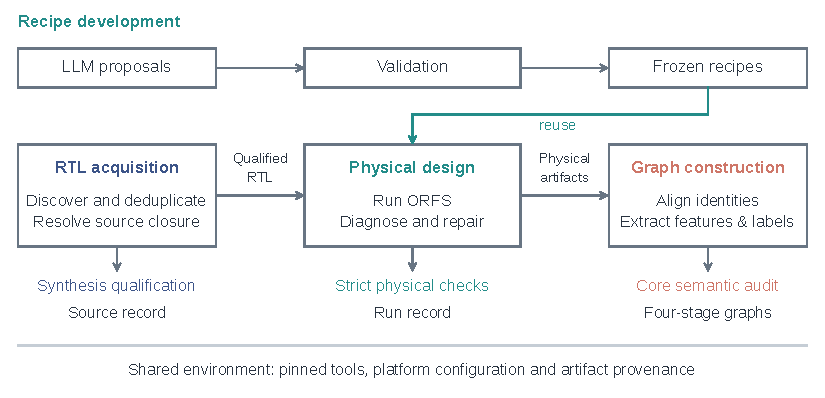
\includegraphics[width=\linewidth]{figures/workflow.pdf}
\caption{R2G workflow and evidence handoffs. A pinned execution environment supports source qualification, physical implementation, and graph construction. Validated repair proposals form frozen recipes for reuse; source, run, and graph records preserve provenance across module boundaries.}
\label{fig:workflow}
\end{figure}

A source record binds repository, commit, top module, compilation inputs, source hashes, and license evidence. A physical run binds configuration, toolchain, stage artifacts, and checking reports. A graph record binds its input artifacts, canonical entity mapping, feature cutoff, label sources, and validation results. These bindings support traceable acceptance decisions and distinguish method failures, unavailable dependencies, and incomplete runs.

The four-stage product incorporates the versioned R2G2.0 builder and recorded integration changes. Its prediction-stage contract is distinct from the five layout views in the prior R2G benchmark~\citep{r2gbenchmark}; code lineage and integration deltas are retained in the artifact documentation.

\subsection{Adaptive Control and Run History}
The operating workflow observes structured candidate records, stage status, failure signatures, physical checks, and graph reports. Admissible decisions include selecting or retrying a candidate, promoting a synthesis-qualified project into physical implementation, applying a scoped repair, resuming an affected stage, scheduling a controlled trial, or escalating a nonconvergent case. Deterministic programs execute these actions and record outcomes. ``Agentic'' describes this observation--decision--execution organization. RTL acquisition and held-out recipe reuse operate without external LLM calls.

The engineer-loop implementation maintains an append-only ledger with pending, flow, signoff, fixing, clean, escalated, and abandoned states. Stage reuse is tied to recorded artifact lineage. Run histories retain failures as well as successes, so recovery does not erase the original outcome. The operational recipe machinery supports candidate, promoted, and shadow states, including evidence-based withdrawal from learned retrieval. Static bootstrap strategies and learned indexed recipes have distinct eligibility paths. The repair experiment evaluates the frozen promotion-and-reuse protocol below.

\subsection{Run-Consistent Dataset Admission}
Physical eligibility and graph validity are distinct requirements. The signoff gate checks backend completion, the required checking reports, and recorded lineage rather than inferring eligibility from a final DEF alone. Its strict mode accepts the exact verdict \texttt{pass}; \texttt{pass\_with\_caveats} belongs to a separate research profile. The required checks and platform capabilities are declared before a campaign.

The complete corpus contract can be expressed as
\begin{equation}
A(d)=Q(d)\land P(d)\land H(d)\land N(d)\land C(d),
\end{equation}
where $Q$ is source qualification, $P$ the declared physical acceptance, $H$ consistent artifact identity and provenance, $N$ native graph validity, and $C$ the implemented core semantic acceptance. Optional label gaps remain explicit in masks and coverage reports; acceptance requires all declared predicates. The conversion experiment evaluates $N$ and $C$ on complete strict-clean physical inputs.

\subsection{Source Qualification}
The acquisition engine discovers repositories, resolves revisions and candidate tops, recovers compilation closure, and forms certified snapshots. The importer checks snapshot and source bindings before synthesis. Deterministic selection limits repository concentration and removes duplicate design families. In the formal acquisition task, each method requests 200 unique designs, with at most four candidates per repository.

Let $q(c)$ indicate whether candidate $c$ passes the frozen qualification rules. These require reproducible source retrieval, a valid top and compilation closure, successful Sky130HD synthesis, a nonempty resolved netlist, $100\leq n_{\mathrm{cells}}<100000$, uniqueness, provenance, and accepted license evidence. The primary yield is
\begin{equation}
Y_{\mathrm{RTL}}=\frac{1}{200}\sum_{c\in\mathcal{S}}q(c),
\end{equation}
where $\mathcal{S}$ is the locked submission. Unfilled slots contribute zero. Submission precision uses $|\mathcal{S}|$ as its denominator and is reported separately. This acquisition gate evaluates synthesis qualification; physical acceptance is evaluated at the subsequent run boundary.

\subsection{Frozen Repair Knowledge}
The repair study separates proposal, validation, and deployment. On the proposal split, LLMs suggest structured configuration actions. Schema and action-policy checks reject invalid parameters, no-ops, and forbidden constraint changes. Admitted candidates must provide useful proposal-split evidence, retain complete provenance, and avoid clean-sentinel regressions. Each executable payload is hashed; exploration outcomes do not themselves count as promotion votes.

After freezing a candidate, formal proposal-split replays and disjoint validation trials provide lifecycle evidence. Let $W$ and $L$ be independent-family wins and losses, $W_v$ validation wins, and $R$ indicate a clean-sentinel regression. The operational promotion rule is
\begin{equation}
\mathrm{promote}(c)=[W\geq2]\land[W>L]\land[W_v\geq1]\land[\neg R].
\end{equation}
Incomplete and inconclusive evidence contributes no promotion vote. Repeated trials from the same RTL family do not provide independent votes. Records with at least two validation wins receive an additional strict-validation-support annotation.

Deployment compares M0 (no learned strategy), M1 (admitted bank in fixed order), M2 (the same bank ranked using A-only evidence), and M3 (promoted recipes only). M1 and M2 attempt at most three candidates per challenge. M2 combines wins, losses, strict-clean outcomes, bounded DRC and WNS gains, and elapsed time in a frozen heuristic; it is not a trained ranking model. M3 abstains when no recipe applies. During held-out deployment, these methods cannot call an LLM, update the bank, or promote a new recipe. The action policy prohibits changing the clock, SDC, footprint, utilization, or signoff check set.

We distinguish overall repair rate $S/N$, policy coverage $C/N$, and conditional success $S/C$. We report all three alongside trial counts to characterize both successful reuse and policy abstention.

\subsection{Four Prediction-Stage Graphs}
For design $d$, the graph builder constructs
\begin{equation}
G_{d,s}=(V_d,E_d,X_{d,s},Y_d,M_d),
\end{equation}
where $V_d$ and logical relations $E_d$ are defined by the canonical post-synthesis netlist. Node types are gates, pins, nets, and I/O pins; core relations are gate--pin membership, pin--net connectivity, and I/O--net connectivity. Features $X_{d,s}$ obey the stage cutoff. Shared post-route labels $Y_d$ retain physical units and explicit validity masks $M_d$.

\begin{table}[htbp]
\caption{Prediction stage and permitted physical inputs. All stages share post-route supervision, which is excluded from encoder inputs.}
\label{tab:cutoff}\centering
\begin{tabular}{lll}\toprule
Graph & Input cutoff & Physical features\\\midrule
Floorplan & Post-synthesis & None\\
Placement & Post-floorplan & Die, I/O, fixed macros\\
CTS & Post-placement & Trusted placement geometry\\
Route & Post-CTS & Trusted CTS geometry\\\bottomrule
\end{tabular}
\end{table}

The node universe remains fixed across stages. A synthesis gate removed by backend optimization remains represented with invalid physical-placement information. Physical net changes are aligned to the canonical topology rather than silently replacing it. Label values satisfy $\mathrm{isfinite}(Y_d)=M_d$; unavailable measurements remain missing, not zero. Timing and RC relations are supervision-only. Their presence as stored relations does not authorize their use in message passing. Geometry relations are permitted only at the CTS and route prediction cutoffs.

\textbf{Joining physical evidence to canonical entities.} R2G uses native Yosys parsing to elaborate bit-level connectivity and normalize escaped identifiers. Assembly joins features and labels by instance, instance--pin, net, and I/O identities, checking key sets before assigning tensor rows and edge indices. Physical extraction then preserves the meaning of each source: routed DEF segments provide wirelength in micrometers after DBU conversion; SPEF names and capacitance units map ground capacitance to canonical nets in pF; STA endpoints map setup/hold slack to canonical pins in ns. These joins carry validity and provenance into the graph. A missing measurement remains masked rather than becoming a zero-valued training target. This design makes topology, physical features, and supervision refer to the same circuit entities.

\subsection{Independent Acceptance Checks}
Native validation checks the output contract, immutable configuration, and structural consistency. An additional oracle checks seven groups: alignment, causal restrictions, identity, labels, masks, numerical features, and topology. Identity and core connectivity are compared with native Yosys parsing. Coordinate checks use OpenDB, LEF, and the permitted DEF. Physical-label checks use independently available route, SPEF, and timing endpoints with frozen tolerances.

For an evaluated design, semantic usability requires native acceptance and a pass in every implemented core group. Each check records pass, fail, or unassessable status. The causal group checks prohibited early features and supervision payloads; label checks report independently matched values and coverage. Semantic usability refers to this implemented core audit.

\section{Experimental Evaluation}
\subsection{Protocol and Scope}
We report four completed studies: RTL acquisition, frozen repair transfer, physical-data conversion, and downstream prediction. Each study uses a dedicated cohort and reports its own acceptance endpoint. The acquisition toolchain is pinned to ORFS commit \texttt{a5ff7ef7}, Yosys 0.64, and OpenROAD \texttt{26Q3-318-g6b9d7fb806}; individual campaigns retain their own runtime and protocol manifests. Models are identified by their full version names throughout.

\subsection{Qualified RTL Acquisition}
Each method receives four CPU cores, one concurrent synthesis job, and a 48-hour wall-clock ceiling. Tool-enabled vanilla LLMs additionally have ceilings of 20 million tokens, 1,600 turns, and 960 search requests. The LLM roster is GPT-5.6-sol, Claude Opus 5, Qwen3.7-Max, Kimi-K2.7-Code, DeepSeek-V4-Pro, grok-4.5, and Gemini-3.1-Pro-Preview. R2G starts with empty search-scheduling state and uses no external LLM tokens. All methods are evaluated after their submissions are locked, using fresh source retrieval and independent synthesis. Confirmed infrastructure failures can be retried on unchanged submissions; actual qualification failures cannot be replaced after scoring.

\begin{figure}[htbp]
\centering
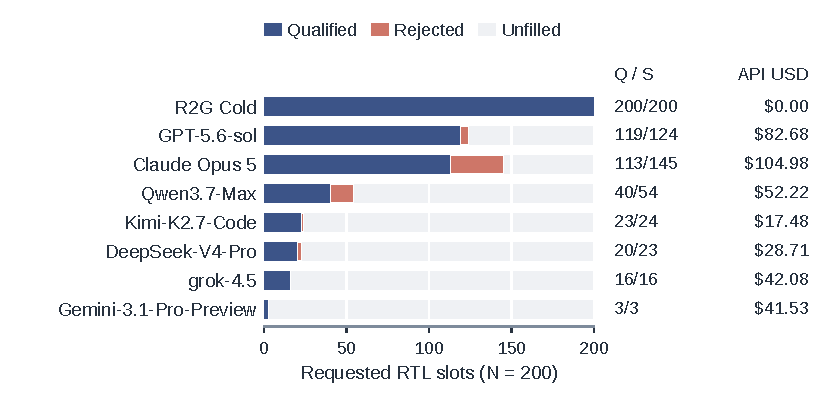
\includegraphics[width=\linewidth]{figures/acquisition_yield.pdf}
\caption{Qualified RTL acquisition under the campaign budgets. Each bar represents 200 requested slots; Q/S gives qualified/submitted counts. Coral denotes rejected submissions; gray denotes unfilled slots. R2G takes 33.52 h. API USD gives reference-price estimates (Appendix~\ref{app:api_costs}).}
\label{fig:acquisition}
\end{figure}

R2G supplies all 200 qualified designs, exceeding GPT-5.6-sol by 81 designs, or 40.5 percentage points of fixed-target yield (Fig.~\ref{fig:acquisition}). Its qualified set spans 122 repositories, compared with 70 for GPT-5.6-sol and 52 for Claude Opus 5, with a maximum single-repository contribution of 2\%. The acquisition bottleneck is not solely submitted-candidate accuracy: GPT-5.6-sol qualifies 119 of 124 submissions, yet leaves 76 slots unfilled. Results are measured per budgeted acquisition campaign.

R2G completes the target in 33.52 hours. The recorded LLM runs take 2.28--10.58 hours and stop at token or turn ceilings, so the comparison measures final qualified yield under the stated budgets. Infrastructure-only reevaluation raises R2G's count from 195 to 200 using the same five submissions; equivalent retry rules apply to the other methods.

\subsection{Repair Transfer and Full-System Evaluation}
The repair cohort contains six proposal challenges, six validation challenges, and 13 held-out challenges: seven DRC and six setup-timing cases. Four baseline-clean sentinels are separate from the repair denominator. Splits prohibit shared repositories, forks, compilation closures, or RTL lineages across subsets. M0--M3 use the prescribed development split; Full R2G uses the complete Recipe library, including recipes developed using evidence from the evaluated challenge set. Every ORFS trial uses four cores and a 7,200-second ceiling at fixed Sky130HD, 100 MHz. GPT-5.6-sol, Claude Opus 5, and Qwen3.7-Max repair each held-out challenge independently with the same permitted actions, up to three response turns and 20,000 tokens per model per challenge.

\begin{figure}[htbp]
\centering
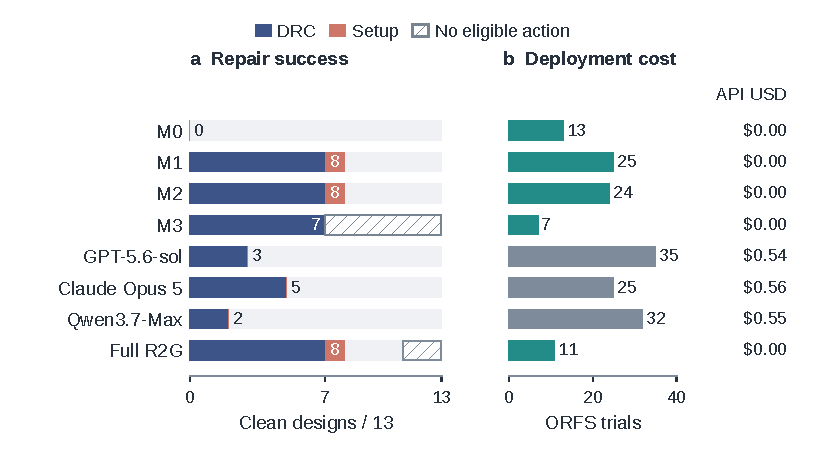
\includegraphics[width=\linewidth]{figures/repair_outcomes_cost.pdf}
\caption{Repair outcomes and deployment cost. Blue/coral count DRC/setup successes out of 13 challenges; gray denotes unsuccessful attempts and hatching no eligible action. Trial counts and estimated API USD cover deployment; the shared proposal phase costs \$0.57 (Appendix~\ref{app:api_costs}).}
\label{fig:repair}
\end{figure}

Seventeen structured records produce ten admitted candidates and three promoted records, corresponding to two distinct executable recipes. Both target the \texttt{DRC:m3.2} edge-pin congestion family: one excludes right-edge pin placement; the other combines hierarchical synthesis with top-edge exclusion. No setup-timing candidate is promoted.

M1 and M2 each repair eight held-out challenges, three more than the strongest pure LLM baseline, Claude Opus 5 (Fig.~\ref{fig:repair}). They reach the same successful design set, with M2 using 24 trials and M1 using 25. M3 repairs seven of 13 challenges overall and seven of seven covered challenges, using one trial per covered case. The promoted policy uses seven trials and abstains on the six setup challenges. M1, M2, and M3 retain strict-clean outcomes on all four tested sentinels.

M1/M2 require 40,460.063/40,919.486 accumulated EDA seconds on the held-out challenges; M3 requires 6,500.894 seconds. These costs sum the individual trial durations. Held-out R2G execution consumes no LLM tokens, but the proposal phase costs 109,236 tokens and 18 calls. The formal A replays also consume 110 ORFS attempts (77 proposal and 33 validation attempts), excluding other learning work. Learning and deployment costs are accounted for separately. The pure-LLM held-out runs consume 207,442 tokens in aggregate.



These results characterize transfer on the seven DRC and six setup challenges. An exploratory paired comparison of M1 and Claude Opus 5 gives three wins unique to M1 and none unique to Claude Opus 5 (two-sided exact McNemar $p=0.25$).

\textbf{Full R2G.} We evaluate a frozen snapshot of the complete native Recipe library on the same 13 challenges, preserving RTL, clock, floorplan, and strict checks. Native ranking and lifecycle gates select actions through the budgeted configuration adapter. Full R2G achieves \textbf{8/13 strict-clean designs (61.54\%)}: seven DRC and one setup case, using \textbf{11 repair trials} with no evaluation-time LLM calls or online learning (Fig.~\ref{fig:repair}). All eight successes occur on the first attempt; two designs have no eligible action and remain in the denominator. Appendix~\ref{app:full_r2g} gives the per-design results and a configuration-only timing repair.

\subsection{From Connectivity to Physically Grounded Graphs}
\label{sec:e4}
\textbf{Progressive development protocol.} Three LLMs start from empty programs and incrementally edit converters using the same six development designs, public graph contract, native Yosys/OpenROAD interfaces, and per-round semantic feedback. Feedback covers entity and edge matching, physical values, labels, masks, stage restrictions, and packaging. Programs execute without network access and cannot read R2G source or other designs' outputs. Each model's initial 400,000-token allocation is extended once to a cumulative 600,000-token ceiling before testing, with at most 18 responses and 16,384 output tokens per response. Code, feedback, and usage carry forward across the extension. GPT-5.6-sol, Claude Opus 5, and Qwen3.7-Max receive 16, 11, and 15 responses and record 556,437, 587,522, and 570,956 effective tokens, respectively; these ledger totals exclude unknown charges for unanswered network requests.

Selection uses development results, ordered by complete semantic passes, identity F1, topology F1, label coverage, feature coverage, and static coverage; ties retain the earlier program. The selected converters and frozen R2G runtime are evaluated on the same 24 strict-clean physical designs from independent source origins, with eight designs in each of three size strata. Every conversion has a 3,600-second ceiling. This is a fixed-benchmark retest of the existing cohort. Structured feedback is restricted to development designs, and test evaluation involves no model calls or subsequent program changes. R2G is an established implementation; the budget controls the LLM development runs, not R2G's historical engineering effort.

\textbf{Metrics.} Complete core acceptance requires all seven semantic groups to pass for a design. Identity and topology F1 are averaged over applicable audited checks across stages and designs. Feature denotes audited numerical inputs: die geometry, gate/pin coordinates, net HPWL, and bounding-box dimensions. Numerical feature correct coverage (Feature) and label correct coverage (Label) average the per-check fraction of expected values that are matched within tolerance. Failed or unassessable checks without a usable denominator contribute zero; passing empty or inapplicable checks are omitted. These are check-level diagnostic aggregates, not percentages of fully correct designs or all possible graph features. Appendix~\ref{app:e4} gives the exact aggregation and status breakdown.

\begin{figure}[htbp]
\centering
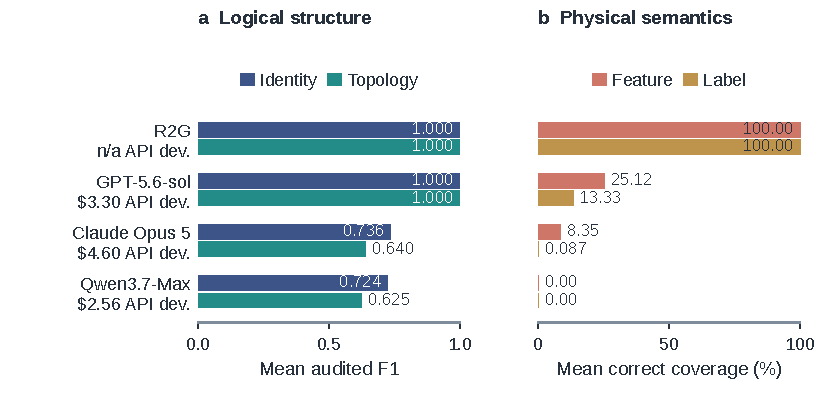
\includegraphics[width=\linewidth]{figures/conversion_semantics.pdf}
\caption{Fixed 24-design conversion benchmark after development under a 600k-token ceiling. Left: identity/topology F1; right: feature/label correct coverage. Model labels include estimated development API USD (Appendix~\ref{app:api_costs}); n/a denotes unmetered tool development. Core acceptance is 24/24 for R2G and 0/24 for each LLM converter.}
\label{fig:conversion}
\end{figure}

\textbf{Topology is necessary but insufficient.} All 96 method--design evaluations complete. R2G passes every core group on all 24 designs, with 1.0 identity/topology F1 and 100\% correct coverage within the audited scope (Fig.~\ref{fig:conversion}). GPT-5.6-sol also attains identity and topology F1 of 1.0; its alignment, mask, and selected causal checks pass on all 24 designs. Its feature and label groups fail on every design, with mean correct coverage of 25.12\% and 13.33\%. Claude Opus 5 reaches identity/topology F1 of 0.7364/0.6400, with 8.35\% feature and 0.087\% label coverage. Qwen3.7-Max reaches 0.7239/0.6247 F1 but provides no verified feature or label coverage. Thus the result distinguishes actual progress in logical reconstruction from completion of the physical supervision interface.

The practical value is an inspectable connection from heterogeneous EDA files to graph inputs and supervision: recovering connectivity alone does not supply stage-valid physical features or correctly associated targets. R2G delivers this connection under the evaluated contract. Appendix~\ref{app:e4} reports development trajectories, detailed check states, and a traced conversion case.

\subsection{Downstream Utility of Stage-Aware Physical Graphs}
\label{sec:downstream}
We test whether the admitted graph fields carry predictive signal rather than merely satisfying a schema. The cohort contains 278 strict-clean designs with a fixed, design-disjoint train/validation/test split of 175/49/54. All reported results use the same 54-design test set and three seeds. GINE models consume topology and numerical features; feature-only MLPs provide a matched non-message-passing baseline. Inputs are restricted to one of four cutoffs---post-synthesis, post-floorplan, post-placement, or post-CTS---and predict common post-route targets. Neither post-route labels nor supervision-only relations enter the encoders. We report test macro MAE, for which lower is better.

\begin{figure}[htbp]
\centering
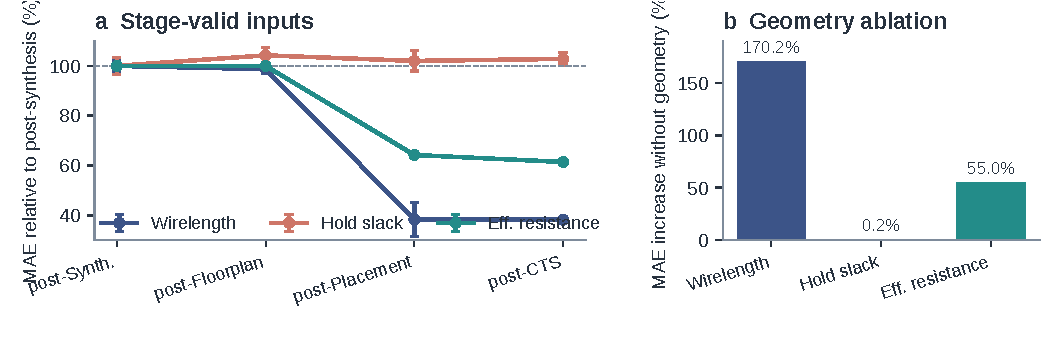
\includegraphics[width=\linewidth]{figures/downstream_utility.pdf}
\caption{Downstream evidence from the fixed 278-design cohort (mean and standard deviation over three seeds). (a) Stage-valid inputs predicting post-route targets, normalized to post-synthesis MAE. (b) Removing geometry from otherwise identical post-placement GINE inputs. Physical stage and geometry information strongly affect wirelength and effective resistance; hold slack is comparatively insensitive.}
\label{fig:downstream}
\end{figure}

Figure~\ref{fig:downstream} shows a sharp information boundary at placement. From post-synthesis to post-placement inputs, wirelength MAE falls from 12.8650 to 4.9321 (61.7\%) and effective-resistance MAE from 14.3060 to 9.1870 (35.8\%). Post-CTS inputs further reach 4.9112 and 8.7820. Removing geometry from post-placement graphs reverses these gains: wirelength MAE rises to 13.3268 (170.2\%) and resistance to 14.2431 (55.0\%). The negligible 0.2\% hold-slack change is an informative negative control rather than evidence of universal benefit.

Topology is likewise target dependent. At post-placement, GINE improves wirelength MAE over the MLP from 7.1548 to 4.9321 and hold-slack MAE from 0.1412 to 0.1316; at post-CTS it improves them from 10.1386 to 4.9112 and from 0.1395 to 0.1327. The MLP is stronger on the other five audited targets. Thus the result is not that one architecture always wins: R2G preserves enough aligned topology, geometry, and supervision to expose which physical targets benefit from each inductive bias.

\section{Discussion}
The studies establish complementary acceptance boundaries. Acquisition supplies qualified sources; frozen repair reuse converts development evidence into executable actions. The converter baseline shows that perfect audited topology can still omit physical values and supervision. R2G connects these layers through canonical identity, unit-aware extraction, stage visibility, and explicit validity. Downstream results close the evidence chain: geometry materially improves wirelength and resistance prediction, whereas hold slack is insensitive and feature-only models outperform GINE on several targets. Rather than claiming universal model dominance, the data support controlled tests of when topology and geometry matter.

\textbf{Reproducibility.} The fixed split, three-seed checkpoints, predictions, and per-design metrics are archived; a local rescore reproduces all 142,996 targets in a representative test run within cross-device tolerance.

\paragraph{Conclusion.} R2G connects qualified acquisition, frozen repair knowledge, and physically grounded graph construction through evidence contracts. It supplies 200 qualified sources, repairs eight of 13 held-out challenges, passes all core audits on 24 conversion designs, and produces stage-aware graphs with measurable physical signal: an auditable path from public RTL to aligned topology, geometry, and supervision.

\label{sec:main_end}
\subsection*{AI use statement}
Generative AI tools assisted with research framing, feedback on experimental methodology, interpretation of reported results, literature search and synthesis, manuscript drafting and editing, and preparation of plotting code and LaTeX artifacts. The experiments also use LLMs explicitly as evaluated acquisition baselines, repair-proposal generators, and converter developers, as described in the evaluation protocols. Manuscript figures are derived from recorded experimental results; source digests and automated numerical and document checks are retained in the artifact records. The authors retain responsibility for the scientific claims, references, code, and reported results.

\bibliography{references}
\bibliographystyle{iclr2027_conference}
\appendix
\section{Conversion Metrics and Development Evidence}
\label{app:e4}
\subsection{Audit aggregation}
For an identity or topology check, the reported F1 is $2TP/(2TP+FP+FN)$. Empty reference/output pairs are excluded when passing; failed or unassessable checks without entity counts receive zero. For a numerical feature or label check with $e>0$ expected values, correct coverage is $\min(1,\max(0,m-i)/e)$, where $m$ is the number of matched values and $i$ the number of matched values outside tolerance. If a failed or unassessable check has no usable expected count, its score is zero; empty passing and inapplicable checks are excluded. Each metric is the arithmetic mean over the included checks from all stages and designs. Repeated stage labels therefore contribute repeated checks; the unique route-endpoint counts in the main text count each design's route labels once. The complete semantic-pass count is computed independently from design-level core verdicts.

\begin{table}[htbp]\centering
\caption{Exact aggregate results for the 600k-budget fixed-cohort retest. Feature/label columns are mean correct coverage under the aggregation above.}
\setlength{\tabcolsep}{3pt}
\begin{tabular}{lrrrrr}\toprule
Method & Core pass & Identity F1 & Topology F1 & Feature & Label\\\midrule
\textbf{R2G} & \textbf{24/24} & \textbf{1.0000} & \textbf{1.0000} & \textbf{100.00\%} & \textbf{100.000\%}\\
GPT-5.6-sol & 0/24 & 1.0000 & 1.0000 & 25.12\% & 13.334\%\\
Claude Opus 5 & 0/24 & 0.7364 & 0.6400 & 8.35\% & 0.087\%\\
Qwen3.7-Max & 0/24 & 0.7239 & 0.6247 & 0.00\% & 0.000\%\\
\bottomrule\end{tabular}

\end{table}

\begin{figure}[htbp]\centering
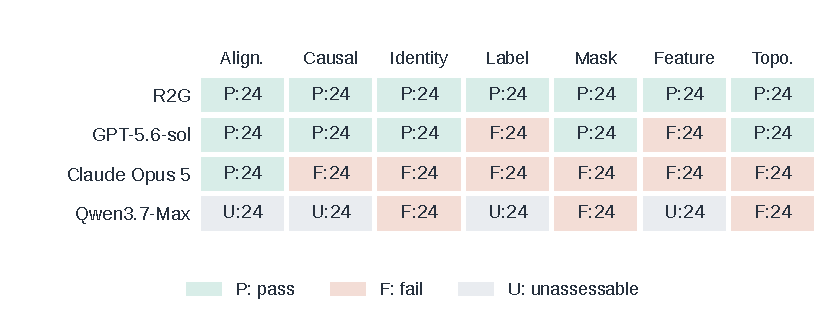
\includegraphics[width=\linewidth]{figures/conversion_core_checks.pdf}
\caption{Design counts in the seven core audit groups. Pass, fail, and unassessable are retained separately. A failure or missing schema may affect several dependent checks; these groups are not independent root causes.}
\end{figure}

The absolute tolerances include 0.0011~$\mu$m for wirelength, $10^{-9}$~pF for ground capacitance, and 0.011~ns for slack, with relative tolerance $10^{-5}$. The audit covers independently available endpoints, not all Liberty attributes, parasitic relations, or physical-label variants.

\subsection{Development budget extension}
The 400k and 600k snapshots below use the same six development designs and the same cumulative development trajectory. They are development metrics, not a comparison of test-set accuracy at two budgets. The 400k snapshots were not retested in this experiment.

\begin{table}[htbp]\centering
\caption{Selected development-program metrics before and after the uniform budget extension. Each arrow denotes 400k $\rightarrow$ 600k ceilings; actual ledger usage can be below the ceiling.}
\setlength{\tabcolsep}{3pt}
\begin{tabular}{lrrrr}\toprule
Model & Identity F1 & Topology F1 & Feature (\%) & Label (\%)\\\midrule
GPT-5.6-sol & 1.000 $\to$ 1.000 & 1.000 $\to$ 1.000 & 18.13 $\to$ 24.80 & 0.000 $\to$ 13.650\\
Claude Opus 5 & 0.684 $\to$ 0.684 & 0.594 $\to$ 0.594 & 8.11 $\to$ 8.11 & 0.118 $\to$ 0.118\\
Qwen3.7-Max & 0.672 $\to$ 0.672 & 0.054 $\to$ 0.577 & 0.00 $\to$ 0.00 & 0.000 $\to$ 0.000\\
\bottomrule\end{tabular}

\end{table}

GPT-5.6-sol improves physical coverage, while Qwen3.7-Max improves topology; Claude Opus 5 retains the same selected program. Additional development can therefore improve individual components without yet completing the graph contract. The main comparison uses one selected program per model, evaluated on all 24 fixed test designs. Test-case diagnosis is performed only after scoring and does not revise these programs or results.

\subsection{Traced conversion case}
Post-test inspection of the selected programs and the \texttt{blinking} design explains the gap between topology and physical supervision (Table~\ref{tab:e4case}). GPT-5.6-sol matches all 211 gates and 644 pins, but none of the 27 expected setup or 27 hold endpoints. Its timing parser primarily expects a slack-before-value pattern, whereas the report contains value-before-slack records such as \texttt{8.54 slack (MET)}; its endpoint resolver also expects an instance/pin form where a report may name only the register instance. These are extraction and joining gaps after successful topology recovery.

\begin{table}[htbp]
\centering
\caption{Representative \texttt{blinking} route-graph audit. Gates/pins show matched identities over expected identities. Label columns show matched values within tolerance over independently expected endpoints. U means unassessable.}
\label{tab:e4case}
\setlength{\tabcolsep}{3pt}
\begin{tabular}{lrrrrrr}\toprule
Method & Gates & Pins & Wirelength & Ground cap. & Setup & Hold\\\midrule
\textbf{R2G} & \textbf{211/211} & \textbf{644/644} & \textbf{209/209} & \textbf{207/207} & \textbf{27/27} & \textbf{27/27}\\
GPT-5.6-sol & 211/211 & 644/644 & 178/209 & 100/207 & 0/27 & 0/27\\
Claude Opus 5 & 184/211 & 563/644 & 2/209 & 0/207 & 0/27 & 0/27\\
Qwen3.7-Max & 184/211 & 466/644 & U & U & U & U\\
\bottomrule\end{tabular}

\end{table}

Claude Opus 5 and Qwen3.7-Max each miss 27 register instances with escaped or special names; their matched pin counts fall to 563 and 466. Missing entities also remove dependent edges. Claude Opus 5's zero initialization produces incorrect physical values and stage-ineligible finite fields; Qwen3.7-Max's missing schemas block physical and label evaluation. R2G preserves all reference identities and matches all independently expected labels in this case: 209 wirelengths, 207 ground capacitances, and 27 values each for setup and hold. Across the 24 designs, the route-graph audit matches 54,322 wirelengths and 54,038 ground capacitances, plus 9,250 values each for setup and hold. The covered wirelength and capacitance endpoints account for 92.3\% and 91.2\% of finite graph values; the remaining values are outside this audit's coverage.

\section{Full R2G: Protocol and Per-Design Results}
\label{app:full_r2g}
\textbf{Protocol.} Full R2G evaluates a frozen snapshot of the complete native Recipe library. It uses native ranking, lifecycle gates, and the fixed-task action policy through the repair study's budgeted configuration adapter. The original 13 designs, RTL sources, 100 MHz clock, fixed die/core, and strict checking set are preserved. One worker uses four CPU cores, with at most three attempts per design and a 7,200-second limit per attempt. Each attempt starts from baseline; successful designs stop, and attempted strategies or duplicate action effects are excluded. Evaluation performs no LLM calls or online learning.

\begin{table}[htbp]\centering
\caption{Full R2G per-design results. All 13 designs remain in the denominator, including two with no eligible action. The three unsuccessful attempted designs retain setup violations; \texttt{blake2s\_core} also introduces DRC violations.}
\label{tab:full_r2g_cases}
\setlength{\tabcolsep}{5pt}
\begin{tabular}{llrl}\toprule
Design & Type & Trials & Outcome\\\midrule
\texttt{aes\_192} & DRC & 1 & Strict clean\\
\texttt{des\_top} & DRC & 1 & Strict clean\\
\texttt{seqcordic} & DRC & 1 & Strict clean\\
\texttt{timer\_top} & DRC & 1 & Strict clean\\
\texttt{reg\_file} & DRC & 1 & Strict clean\\
\texttt{wbuart} & DRC & 1 & Strict clean\\
\texttt{picorv32} & DRC & 1 & Strict clean\\
\texttt{blake2s} & Setup & 0 & No eligible action\\
\texttt{iir\_biquad\_axis} & Setup & 1 & Strict clean\\
\texttt{blake2s\_core} & Setup & 1 & Setup violations remain\\
\texttt{tanh} & Setup & 0 & No eligible action\\
\texttt{fft8\_stream} & Setup & 1 & Setup violations remain\\
\texttt{pipelined\_iir} & Setup & 1 & Setup violations remain\\
\midrule
\textbf{Total} & 13 designs & \textbf{11} & \textbf{8 strict clean}\\
\bottomrule\end{tabular}

\end{table}

\textbf{Configuration-only timing repair.} Seven DRC trials rebalance pin placement; four setup trials combine hierarchical synthesis with placement timing repair using \path|SYNTH_HIERARCHICAL=1| and \path|ENABLE_PLACE_REPAIR_TIMING=1|. Without RTL edits, \texttt{iir\_biquad\_axis} improves setup WNS from $-2.69817$ to $+0.106265$ ns, a $2.804435$ ns gain. Final hold WNS is $+0.4358$ ns, with zero DRC, LVS, route, and antenna violations. The stored recipe therefore resolves a setup failure while retaining the registered source and physical constraints.

\textbf{Outcome and cost accounting.} Eight of 11 trials succeed, all on the first attempt; design success is $8/13=61.54\%$. Attempt durations sum to 19,296.617 seconds, excluding baseline, recipe development, and later exploration. This is accumulated trial time, not campaign wall time. Trial-count comparisons describe deployment effort under different knowledge histories, not total development cost or an isolated mechanism effect. This arm did not rerun the four clean sentinels; their earlier M1--M3 outcomes are not attributed to Full R2G. Later source rewrites and out-of-policy experiments are excluded.

\section{API Cost Accounting}
\label{app:api_costs}

Dollar annotations use recorded token consumption and official public prices checked on September 17, 2026. They express a common \emph{uncached, base-context reference-price convention}, using standard inference and excluding cache/batch discounts, long-context and regional premiums, taxes, EDA compute, and engineering time. Thus, they compare the API resource requirements of the reported campaigns rather than reconstructing intermediary invoices. For input tokens $T_{\mathrm{in}}$, generated tokens $T_{\mathrm{out}}$, and prices per million tokens $p_{\mathrm{in}},p_{\mathrm{out}}$, we compute
\[
 C_{\mathrm{API}} = \bigl(T_{\mathrm{in}}p_{\mathrm{in}} + T_{\mathrm{out}}p_{\mathrm{out}}\bigr)/10^6.
\]
The acquisition runner records visible output and reasoning separately; both contribute to $T_{\mathrm{out}}$. Repair and converter-development ledgers already include reasoning in completion counts, which we count once.

\paragraph{Reference prices.}
Input/output USD per million tokens are
\href{https://developers.openai.com/api/docs/models/gpt-5.6-sol}{GPT-5.6-sol}: 4/20;
\href{https://platform.claude.com/docs/en/models/opus-5/whats-new-opus-5}{Claude Opus 5}: 5/25;
\href{https://www.alibabacloud.com/help/en/model-studio/qwen3-7-max}{Qwen3.7-Max}: 2.50/7.50;
\href{https://platform.kimi.ai/}{Kimi-K2.7-Code}: 0.95/4;
\href{https://api-docs.deepseek.com/quick_start/pricing/}{DeepSeek-V4-Pro}: 1.32/3.96;
\href{https://docs.x.ai/developers/pricing}{grok-4.5}: 2/6; and
\href{https://ai.google.dev/gemini-api/docs/gemini-3}{Gemini-3.1-Pro-Preview}: 2/12.
Model names link to the official sources. We use Qwen3.7-Max's Singapore international list rate and DeepSeek-V4-Pro's peak rate consistently. The GPT-5.6-sol rate is the published promotion available at least through November 21, 2026. These fixed reference rates do not infer request-level cache hits or pricing tiers from aggregate tokens.

\paragraph{Campaign scope.}
Acquisition annotations cover the recorded acquisition runs. Repair annotations cover the 13 challenge deployments; M0--M3 and Full R2G make no deployment-time LLM calls. The shared proposal phase for M1--M3 costs \$0.57: \$0.19 for GPT-5.6-sol, \$0.22 for Claude Opus 5, and \$0.17 for Qwen3.7-Max (total computed before rounding), across 109,236 tokens and 18 calls. Full R2G's historical library development is outside that proposal ledger. Conversion annotations cover the actual development usage under the 600,000-token ceiling; subsequent 24-design conversion and scoring invoke no LLM. R2G's earlier tool-development cost is unmetered and shown as n/a. A zero API annotation refers only to the indicated execution phase.

\end{document}
